% !TEX program = xelatex
% !TEX spellcheck = en_US

% !TeX TXS-program:compile = txs:///xelatex/[--shell-escape] 

\documentclass{beamer}
\mode<presentation>

\setbeamertemplate{navigation symbols}{}
\setbeamertemplate{theorems}[numbered]
\setbeamertemplate{items}[default]
\setbeamercovered{dynamic}
\setlength{\unitlength}{1cm}
\setbeamertemplate{footline}[frame number]

\usepackage{setspace}
\usepackage{amsmath,amssymb}
\usepackage{amsthm}
\usepackage{pgf,pgfarrows}
\usepackage[utf8]{inputenc}
\usepackage[T1]{fontenc}
%\usepackage{fontspec}
\usepackage{polski}
\usepackage{graphics}
\usepackage{tikz}
\usetikzlibrary{positioning,decorations.pathreplacing}
\usepackage[ruled]{algorithm}
\usepackage{scalefnt}
\usepackage{array}
\usepackage{colortbl}
\usepackage{lipsum}
\usepackage{subcaption}
\usepackage{multicol} 
\usepackage{multirow}
\usepackage[ruled,vlined]{algorithm2e}
%\usepackage{algorithmic}
\usepackage{float}
\usepackage{appendix}
%
\usetikzlibrary{arrows,automata,snakes}
\usetheme{Frankfurt}
\usecolortheme{seahorse} %crane
\useinnertheme{circles}


\newtheorem*{lemat}{Lemat}
\newtheorem{twierdzenie}{Twierdzenie}
\newtheorem{fakt}{Fakt}
\newtheorem{definicja}{Definicja}
\newtheorem{przyklad}{Przykład}
\newcommand{\myitem}{\item[$\vartriangleright$]}
\newcommand{\nota}[1]{{\color{gray} \emph{#1}}}
\newcommand{\HarmonicN}[1]{H_{#1}}
\newcommand{\BALL}[2]{\mathbf{B}(#1,#2)}
\newcommand{\DISC}[2]{\mathbf{D}(#1,#2)}
\newcommand{\SPHERE}[2]{\mathbf{S}(#1,#2)}
\newcommand{\BigO}[1]{\mathcal{O}\left(#1\right)}
\newcommand{\BigTh}[1]{\Theta\left(#1\right)}
\newcommand{\slfrac}[2]{\left.#1\middle/#2\right.}
\newcommand{\PR}[1]{\mathrm{Pr}\left[#1\right]}
\newcommand{\EE}[1]{\mathbb{E}\left[#1\right]}
\newcommand{\var}[1]{\mathbb{V}\mathrm{ar}\left[#1\right]}
\newcommand{\RR}{\mathbb{R}}
\DeclareMathOperator*{\argmax}{arg\,max}
\DeclareMathOperator*{\argmin}{arg\,min}
% Skrócony symbol liczb naturalnych
\newcommand{\NN}{\mathbb{N}}

% Skrócony symbol liczb wymiernych
\newcommand{\QQ}{\mathbb{Q}}

% Skrócony symbol liczb całkowitych
\newcommand{\ZZ}{\mathbb{Z}}

\newcolumntype{C}{>{\centering\arraybackslash}p{0.5cm}}
\newcolumntype{Y}{>{\columncolor{blue!5}}C}

%\pgfpagesuselayout{4 on 1 with notes}[a4paper,border shrink=3mm]


\title{Zastosowanie szkiców danych w analizie dużych grafów}

\author{
	\textbf{Paweł Polerowicz}
	\newline \newline
	Praca napisana pod kierunkiem \textbf{dr. inż. Jakuba Lemiesza}
}

\date{\today}


\begin{document}

\begin{frame}[plain]{}
	\titlepage
\end{frame}


 \section{Wstęp}
 \begin{frame}[squeeze]{Główne sposoby modelowania problemu}
    \begin{itemize}
        \setlength\itemsep{0.6em}
        \item Model klasyczny
        \item Model strumieniowy 
        \item Model półstrumieniowy
        \item Model rozproszony
    \end{itemize}

    \begin{definicja}[Strumień grafowy]
        Strumieniem grafowym nazywamy ciągłą sekwencję elementów, z których każdy ma postać trójki: 
        \[
            e_i = (<s_i, d_i>; w_i, t_i),
        \]
        gdzie $s_i, d_i$ wierzchołki grafu i przez parę $<s_i, d_i>$ oznaczamy krawędź pomiędzy nimi. Z kolei $w_i$ i $t_i$ to odpowiednio waga tej krawędzi i moment jej wystąpienia.
    \end{definicja}
\end{frame}
 \begin{frame}[squeeze]{Cele pracy}
    \begin{itemize}
        \setlength\itemsep{1em}
        \item Przegląd istniejących rozwiązań w dziedzinie analizy strumieni grafowych.
        \item Generowanie zanurzeń wierzchołków.
        \item Użycie schematu szkicowania opartego na próbkach z rozkładu wykładniczego.
        \item Wykorzystanie operacji teoriomnogościowych do efektywnego operowania na szkicach danych.
        \item Analiza precyzji rekonstrukcji krawędzi grafu oraz złożoności obliczeniowej.
    \end{itemize}
\end{frame}

 \section{Zanurzenia wierzchołków}
 \begin{frame}[squeeze]{Zanurzenia wierzchołków}
    \begin{definicja}
        Zanurzeniem wierzchołka $v$ nazywamy wektor $\overline{S}^v \in \mathbb{R}^m_{+}$, wyznaczany na podstawie cech danego wierzchołka. Będziemy przyjmować $m \ll |V|$.
    \end{definicja}

    \begin{itemize}
        \setlength\itemsep{1em}
        \item Zanurzenia wierzchołków stanowią efektywną pamięciowo reprezentację grafu -- złożoność $O(m|V|)$. 
        \item Mogą być tworzone na różne sposoby, np. próbkowanie wierzchołków i spacery losowe, faktoryzacja macierzy sąsiedztwa, \textbf{wykorzystanie funkcji haszujących do generowania próbek z rozkładu wykładniczego}.
        \item Taka reprezentacja może zostać łatwo wykorzystana jako dane w uczeniu maszynowym. 
    \end{itemize}
\end{frame}
 
 \section{Algorytmy}
 \begin{frame}[squeeze]{NodeSketch (Yang, Rosso, Li, Cudre-Mauroux, 2019)}
    \begin{algorithm}[H]
        \small
        \caption{NodeSketch($\tilde{A},k,\alpha$)}\label{alg:node_sketch}
        \uIf{$k > 2$}{
            $S(k-1) \gets NodeSketch(\tilde{A},k - 1,\alpha)$\;
            \ForEach{rząd $r$ w $\tilde{A}$}{
                $\color{black} \tilde{V}_{i}^{r}(k) \gets \tilde{V}_{i}^{r} + \sum\limits_{n \in 	\Gamma(r)} \frac{\alpha}{m} \sum\limits_{j = 1}^{m} \mathbbm{1}_{[S_{j}^{n}(k - 1) = i]}, i \in \{1,2, \dots, D\}$\;\\
                $\color{black} S_{j}^{r}(k) \gets \argmin_{i \in \{1,2,\dots, D\}} \frac{-\log h_{j}(i)}{\tilde{V}_{i}^{r}(k)}, j \in \{1,2, \dots, m\}$\;
            }
        }
        \ElseIf{$k = 2$}{
            \ForEach{rząd $r$ w $\tilde{A}$}{
                $\color{black} S_{j}^{r}(2) \gets \argmin_{i \in \{1,2,\dots, D\}} \frac{-\log h_{j}(i)}{\tilde{V}_{i}^{r}(2)}, j \in \{1,2, \dots, m\}$\;
            }
        }
        \Return{$S(k)$}
    \end{algorithm}

\end{frame}
 \begin{frame}[squeeze]{ExpSketch (Lemiesz, 2021)}
    Metoda generowania próbek dla krawędzi $i$ o wadze $\lambda_i$ w algorytmie \texttt{ExpSketch}:
    \[
        E = - \frac{\ln(h(i || k))}{\lambda_i} \sim Exp(\lambda_i).
    \]

    \begin{twierdzenie}[Suma szkiców]
        Niech $A, B$ - szkice zbiórów $\mathbb{A}, \mathbb{B}$. Wtedy szkic ich sumy możemy wyznaczyć (z własności rozkładu wykładniczego) jako:
        \[
            A \mathbin{\mathaccent\cdot\cup} B = (\min{\{A_1, B_1\}}, \min{\{A_2, B_2\}}, \dots, \min{\{A_m, B_m\}}).
        \]
    \end{twierdzenie}

\end{frame}

\begin{frame}[squeeze]{ExpSketch (Lemiesz, 2021)}
    \begin{definicja}[Ważone podobieństwo Jaccarda]
        Ważone podobieństwo Jaccarda to miara podobieństwa dwóch zbiorów, zdefiniowanae jako stosunek sumy wag elementów wspólnych do sumy wag elementów w sumie mnogościowej zbiorów.
        \[
            J_w(\mathbb{A}, \mathbb{B}) = \frac{|\mathbb{A} \cap \mathbb{B}|_w}{|\mathbb{A} \cup \mathbb{B}|_w}.
        \]
    \end{definicja}

    \begin{twierdzenie}
        Nieobciążony estymator ważonego podobieństwa Jaccarda zbiorów $\mathbb{A}$ i $\mathbb{B}$ można otrzymać, wykorzystując ich szkice:
        \[
            \hat{J}_w(A, B) = \frac{1}{m} \sum\limits_{k = 1}^{m} \mathbbm{1}[A_k = B_k].  
        \]
    \end{twierdzenie}
\end{frame}
 \begin{frame}[squeeze]{EdgeSketch}
    \small
    \begin{algorithm}[H]
        \caption{EdgeSketch($\tilde{A},m$)}\label{alg:edge_sketch}
        \ForEach{\textnormal{rząd} $r$ \textnormal{w} $\tilde{A}$}{
            $ns \gets [\,]$ \tcp*{lista sąsiadów}
            \ForEach{$i \in \{1,\dots,|V|\}$}{
                \If{$\tilde{A}[r,i] \neq 0$}{
                    $ns \gets ns \cup \{((\min(i,r) || \max(i,r)),\tilde{A}[r,i])\}$\;
                }
            }
            $S^{r} \gets FastExpSketch(ns, m)$\;
        }
        \Return{$S$}
    \end{algorithm}

    \begin{lemat}[Złożoność czasowa]
        Złożoność czasowa \texttt{EdgeSketch} wynosi ogółem $O(m(|V|)^2)$, a w średnim przypadku dla grafów nieważonych:
        \[
            O((|V|)^2 + |V|(m \ln(m) \ln(|V|)))
        \]
    \end{lemat}
\end{frame}

\begin{frame}[squeeze]{EdgeSketch}
    \begin{itemize}
        \item Miarą skuteczności algorytmów była precyzja rekonstrukcji krawędzi grafu. 
        \item Rekonstrukcja wierzchołków -- oblicznie macierzy podobieństw Jaccarda zbiorów reprezentujących k-sąsiedztwa wierzchołków i wybór $t$ najwyższych wartości.
        \item Ostateczna macierz podobieństw w algorytmie \texttt{EdgeSketch} powstaje na podstawie macierzy niższych rzędów:
        \[
            simM = \sum\limits_{k = 2}^{K} \alpha^{k-2} simM_{k}.
        \]
        \item W algorytmie \texttt{NodeSketch} jest ona obliczana raz, na podstawie zanurzeń wygenerowanych dla danego $k$.  
    \end{itemize}
\end{frame}

 \section{Wyniki}
 \begin{frame}[squeeze]{Wpływ rozmiaru szkicu na precyzję rekonstrukcji}

    \begin{table}[t]
        \small
        \centering
        \resizebox{\columnwidth}{!}{%
        \begin{tabular}{|l|l|l|l|l|l|l|l|l|l|}
            \hline
            & & \multicolumn{4}{c|}{NodeSketch} & \multicolumn{4}{c|}{EdgeSketch} \\ \cline{1-10}
            \textbf{$b$} & \textbf{k} & \textbf{t = 100} & \textbf{t = 1000} & \textbf{t = 10000} & \textbf{t = |E|} & \textbf{t = 100} & \textbf{t = 1000} & \textbf{t = 10000} & \textbf{t = |E|} \\ \hline\hline
            \multirow{3}{*}{2} & 2 & 0.57 & 0.525 & 0.5136 & 0.5072 & 1 & 1 & 0.4391 & 0.2616 \\ \cline{2-10}
             & 3 & 0.47 & 0.527 & 0.5089 & 0.5016 & 1 & 1 & 0.4545 & 0.3426 \\ \cline{2-10}
             & 4 & 0.44 & 0.523 & 0.5079 & 0.5022 & 1 & 1 & 0.4545 & 0.3426 \\ \hline\hline
            \multirow{3}{*}{4} & 2 & 0.5 & 0.542 & 0.5343 & 0.5131 & 1 & 1 & 0.3352 & 0.1547 \\ \cline{2-10}
             & 3 & 0.53 & 0.483 & 0.4991 & 0.5003 & 1 & 1 & 0.5342 & 0.4087 \\ \cline{2-10}
             & 4 & 0.46 & 0.499 & 0.4983 & 0.5008 & 1 & 1 & 0.5342 & 0.4087 \\ \hline\hline
            \multirow{3}{*}{8} & 2 & 0.66 & 0.594 & 0.5521 & 0.5234 & 1 & 1 & 0.2831 & 0.1289 \\ \cline{2-10}
             & 3 & 0.51 & 0.528 & 0.5158 & 0.5063 & 1 & 0.884 & 0.5825 & 0.4762 \\ \cline{2-10}
             & 4 & 0.5 & 0.496 & 0.5002 & 0.5029 & 1 & 0.884 & 0.5821 & 0.4755 \\ \hline
        \end{tabular}}
        \caption{Precyzja uzyskiwana przez algorytmy NodeSketch i EdgeSketch dla grafów w stochastycznym modelu blokowym dla różnych liczb bloków $b$ oraz wielkości próbek $t$.}
        \label{tab:stochastic_block_model}
    \end{table}
\end{frame}
 \begin{frame}[squeeze]{Wpływ rozmiaru szkicu na precyzję rekonstrukcji}

    \begin{table}[t]
        \small
        \centering
        \resizebox{\columnwidth}{!}{%
        \begin{tabular}{|l|l|l|l|l|l|l|l|l|l|}
        \hline
        & & \multicolumn{4}{c|}{NodeSketch} & \multicolumn{4}{c|}{EdgeSketch} \\ \cline{1-10}
                \textbf{p} & \textbf{k} & \textbf{t = 100} & \textbf{t = 1000} & \textbf{t = 10000} & \textbf{t = |E|} & \textbf{t = 100} & \textbf{t = 1000} & \textbf{t = 10000} & \textbf{t = |E|} \\ \hline\hline
            \multirow{3}{*}{0.0005} & 2 & 0 & 0 & 0.0012 & 0.0031 & 1 & 1 & 1 & 0.5505 \\ \cline{2-10}
            & 3 & 0 & 0 & 0.007 & 0.0248 & 1 & 1 & 0.94 & 0.6125 \\ \cline{2-10}
            & 4 & 0 & 0.006 & 0.0122 & 0.012 & 1 & 1 & 0.9207 & 0.6073 \\ \hline\hline
            \multirow{3}{*}{0.001} & 2 & 0 & 0 & 0.0016 & 0.0055 & 1 & 1 & 1 & 0.3721 \\ \cline{2-10}
            & 3 & 0.01 & 0.017 & 0.012 & 0.006 & 1 & 1 & 0.9671 & 0.4235 \\ \cline{2-10}
            & 4 & 0 & 0.003 & 0.0084 & 0.0099 & 1 & 1 & 0.9714 & 0.4275 \\ \hline\hline
            \multirow{3}{*}{0.005} & 2 & 0.01 & 0.008 & 0.0054 & 0.0065 & 1 & 1 & 1 & 0.0989 \\ \cline{2-10}
            & 3 & 0 & 0.007 & 0.0086 & 0.0063 & 1 & 0.941 & 0.3344 & 0.0581 \\ \cline{2-10}
            & 4 & 0 & 0.004 & 0.0064 & 0.0088 & 1 & 0.941 & 0.3344 & 0.0581 \\ \hline\hline
            \multirow{3}{*}{0.01} & 2 & 0 & 0.01 & 0.0086 & 0.0107 & 1 & 1 & 1 & 0.0583 \\ \cline{2-10}
            & 3 & 0.03 & 0.012 & 0.0101 & 0.0117 & 1 & 1 & 1 & 0.05 \\ \cline{2-10}
            & 4 & 0.01 & 0.011 & 0.0151 & 0.0138 & 1 & 1 & 1 & 0.05 \\ \hline
        \end{tabular}}
        \caption{Precyzja uzyskiwana przez algorytmy NodeSketch i EdgeSketch dla grafów ważonych w modelu Erdosa-Renyiego.}
        \label{tab:weighted_graphs}
    \end{table}
\end{frame}

 \begin{frame}[squeeze]{Wpływ rozmiaru szkicu na precyzję rekonstrukcji}

    \begin{figure}[H]
        \centering
        \begin{minipage}[t]{0.9\textwidth}
            \centering
            \fbox{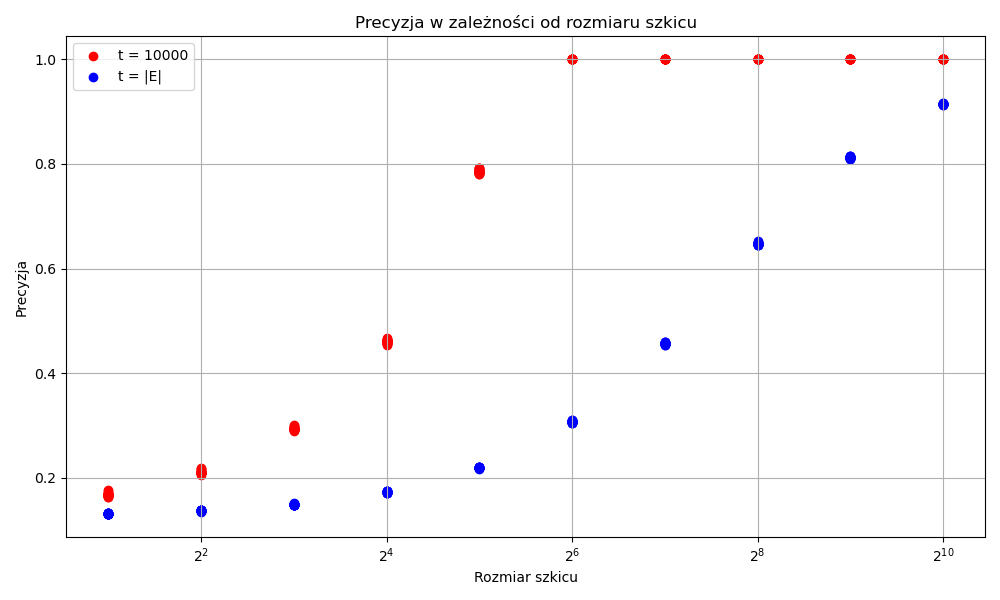
\includegraphics[width=\textwidth]{./img/precision_m.png}}
            \caption{Precyzja uzyskiwana przez algorytm EdgeSketch w zależności od rozmiaru szkicu dla grafu w stochastycznym modelu blokowym.}
        \end{minipage}
    \end{figure} 
\end{frame}
 \begin{frame}[squeeze]{Złożoność obliczeniowa}

    \begin{figure}[H]
        \centering
        \begin{minipage}[t]{0.45\textwidth}
            \centering
            \fbox{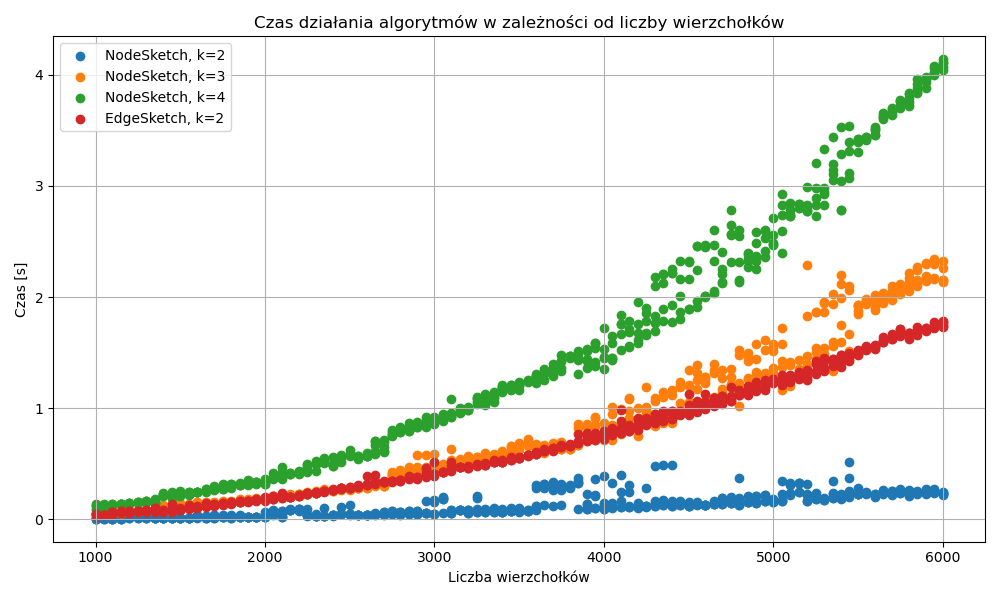
\includegraphics[width=\textwidth]{./img/time_all.png}}
            \caption{Czas działania algorytmów w zależności od liczby wierzchołków.}
        \end{minipage}
        \hspace{0.03\textwidth}
        \begin{minipage}[t]{0.45\textwidth}
            \centering
            \fbox{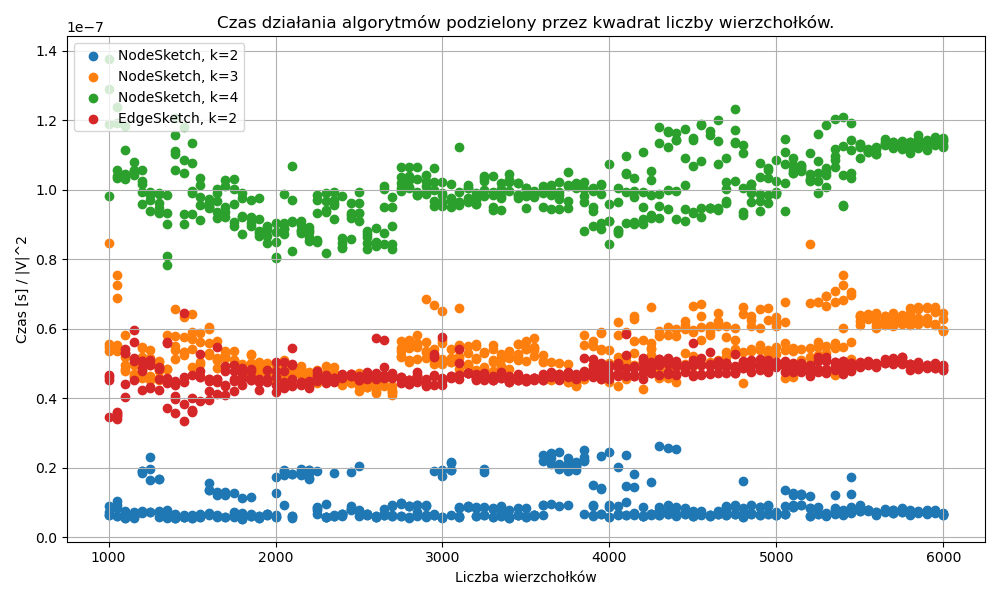
\includegraphics[width=\textwidth]{./img/time_normalized.png}}
            \caption{Czas działania algorytmów podzielony przez kwadrat liczby wierzchołków.}
        \end{minipage}
    \end{figure} 
\end{frame}


\section{}
\begin{frame}{}
	\begin{center}
		\large{Dziękuję za uwagę.}
	\end{center}
\end{frame}

\end{document} 